% Figure from MATH 590 notes, section 3. Compile with the notes preamble.
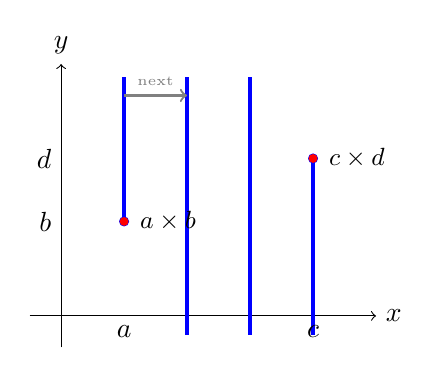
\begin{tikzpicture}[scale=0.8]
    % Axes
    \draw[->] (-0.5,0) -- (5,0) node[right] {$x$};
    \draw[->] (0,-0.5) -- (0,4) node[above] {$y$};
    
    % Shaded region - vertical line at x=a (upper part)
    \draw[very thick, blue] (1,1.5) -- (1,3.8);
    \draw[blue, fill=white] (1,1.5) circle (2pt);
    
    % Shaded region - full vertical lines for a < x < c
    \draw[very thick, blue] (2,-0.3) -- (2,3.8);
    \draw[very thick, blue] (3,-0.3) -- (3,3.8);
    
    % Shaded region - vertical line at x=c (lower part)
    \draw[very thick, blue] (4,-0.3) -- (4,2.5);
    \draw[blue, fill=white] (4,2.5) circle (2pt);
    
    % Points
    \node[below] at (1,0) {$a$};
    \node[below] at (4,0) {$c$};
    \node[left] at (0,1.5) {$b$};
    \node[left] at (0,2.5) {$d$};
    
    % Labels for points
    \fill[red] (1,1.5) circle (2pt);
    \fill[red] (4,2.5) circle (2pt);
    \node[right] at (1.1,1.5) {\small $a \times b$};
    \node[right] at (4.1,2.5) {\small $c \times d$};
    
    % Arrow showing direction
    \draw[->, thick, gray] (1,3.5) to[out=0,in=180] (2,3.5);
    \node[above, gray] at (1.5,3.5) {\tiny next};
\end{tikzpicture}
